\documentclass{article}
\usepackage{graphicx}
\usepackage{amsmath}
\usepackage{xcolor}
\usepackage{tikz}
\usetikzlibrary{automata, positioning, arrows}




\begin{document}

\title{CyberSecurity}
\author{Alessandro Savioli}
\date{November 2024}

\maketitle

\tableofcontents

\newpage

\section{Preface}

The NIST defines the term \textbf{Computer Security} as follows:

\begin{center}
    \textit{Measures and controls that ensure Confidentiality, Integrity, and
    Availability of information system assets including hardware, software,
    firmware, and information being processed, stored, and communicated.}
\end{center}

This definition introduces three key objectives that are the heart of computer
security:

\begin{itemize}
    \item \textbf{Confidentiality}: This term covers two related concepts:
    \begin{itemize}
        \item \textbf{Data Confidentiality}: Assures that private or
        confidential information is not made available or disclosed to
        unauthorized individuals.
        \item \textbf{Privacy}: Assures that individuals control or influence
        what information related to them may be collected and stored and by whom
        and to whom that information may be disclosed.
    \end{itemize}
    \item \textbf{Integrity}: Also this term covers two related concepts:
    \begin{itemize}
        \item \textbf{Data Integrity}: Assures that information and programs are
        \\ changed only in a specified and authorized manner.
        \item \textbf{System Integrity}: Assures that a system performs its
        intended function in an unimpaired manner, free from deliberate or
        inadvertent unauthorized manipulation of the system
    \end{itemize}
    \item \textbf{Availability}: Assures that systems work promptly and service
    is not denied to authorized users.
\end{itemize}

These three concepts form what is often referred to as the \textbf{CIA triad}.
The three concepts embody the fundamental security objectives for both data and
for information and computing services.

Although the use of the CIA triad to define security objectives is well
established, some in the security field feel that additional concepts are needed
to present a complete picture. Two of the most commonly mentioned are as
follows:

\begin{itemize}
    \item \textbf{Authenticity}: The property of being genuine and being able to
    be verified and trusted, confidence in the validity of a transmission, a
    message, or message originator. This means verifying that users are who they
    say they are and that each input arriving at the system came from a trusted
    source.
    \item \textbf{Accountability}: The security goal that generates the
    requirement for actions of an entity to be traced uniquely to that entity.
\end{itemize}

\newpage

\subsection{Tools for Confidentiality}

As we mentioned earlier, Confidentiality is the avoidance of the unauthorized disclosure
of information, it involves the protection of data, providing
access for those who are allowed to see it while
disallowing others for learning about its content.
There are multiple tools to ensure Confidentiality:


\begin{itemize}
    \item \textbf{Encryption}: The transformation of 
    information using a secret, called an \textit{encryption key},
    so that the transformed information can only be read using
    another secret, called the \textit{decryption key}. (Which may, in some cases,
    be the same as the encryption key).

\begin{center}
    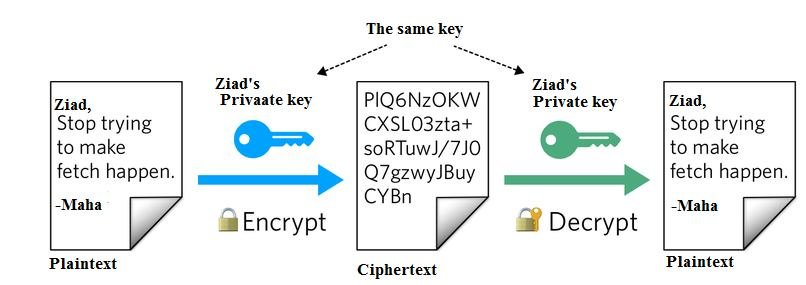
\includegraphics[scale=0.35]{Images/Data-encryption-decryption-process.png}
\end{center}

    \item \textbf{Acces Control}: Rules and policies that limit
    access to confidential information to those people and/or systems
    with a \textbf{Need To Know} determined by identity.
    
    \item \textbf{Authentication}: The determination of the identity or role that someone 
    has. This determination can be done in a number of different ways, but it is usually
    based on a combination of:
    \begin{itemize}
        \item Something the person Has (like a smart card)
        \item Something the person Knows (like a password)
        \item Something the person Is (like a human with the fingerprint)
    \end{itemize}

    \item \textbf{Authorization}: The determination if a person or system is allowed access to 
    resources, based on an access control policy

    \item \textbf{Physical Security}: The establishment of physical barriers to limit
    access to protected computational resources
\end{itemize}

\subsection{Tools for Integrity}

Integrity is the property that something has not be altered in an unauthorized way.

\begin{itemize}
    \item \textbf{Backups}: The periodic archiving of Data
    \item \textbf{Checksums}: The computation of a function that maps the contents of a file 
    to a numerical value. A checksum function depends on the entire contents of a file
    and is designed in a way that even a small change to the input file is highly likely
    to result in a different output value
    \item \textbf{Data correcting codes}: Methods for storing data in such a way
    that small changes can be easily detected and automatically corrected 
\end{itemize}

\subsection{Tools for Availability}

Availability is the property that something is accessible and 
modifiable in a timely fashion by those authorized to do so.

\begin{itemize}
    \item \textbf{Physical protections}: Infrastucture meant to keep information avaible even in the event of physical challenges
    \item \textbf{Computation redundancies}: Computers and storage devices that serve as fallbacks in the case of failures 
\end{itemize}

\subsection{Tools for Authenticity}

Authenticity is the ability to determine that statements, policies and permissions issued by persons or systems are genuine.
 
\begin{itemize}
    \item \textbf{Digital signatures}: These are cryptographic computations that allow a person or system
    to commit to the authenticity of their documents in a unique way that achieves \textbf{non-repudiation}, which is the property 
    that authentic statements issued by some person or system cannot be denied 
\end{itemize}

\section{Threats and Attacks}

\end{document}